\chapter{Advanced Quantum Mechanics Lecture 3: Angular Momentum and Central-Force Reduction\thanks{Lecture notes by Leonard Susskind; transcription curated by LazyingArt LLC}}

Susskind re-centers the lecture by opening the angular sector first, then using it as the organizing bridge into central-force quantum mechanics. The key move is not a bag of formulas but a kinematic strategy: angular degrees of freedom are isolated by angular-momentum representation theory, and each \(\ell\)-sector reduces a three-dimensional differential problem to a one-dimensional radial equation with an \(\ell\)-dependent effective potential.

\section{Angular dependence as angular momentum structure}
For a central potential, translational details are secondary; the problem structure is carried by angle dependence and its generators. In two dimensions, Susskind uses the standard generator form
\[
\hat L_z=-i\hbar\,\frac{\partial}{\partial\phi}.
\]
An eigenstate with angular dependence \(e^{i\ell\phi}\) satisfies
\[
\hat L_z\psi_\ell(\theta,\phi)=\hbar \ell\,\psi_\ell(\theta,\phi),\qquad \ell\in\mathbb Z.
\]
Single-valuedness on \(0\le \phi<2\pi\) enforces \(\ell\in\mathbb Z\).

In three dimensions, the same idea generalizes: angular dependence is packaged by spherical harmonics,
\[
\psi(r,\theta,\phi)=R_\ell(r)\,Y_\ell^m(\theta,\phi),
\]
with quantum data extracted by
\[
\mathbf L^2 Y_\ell^m=\hbar^2\ell(\ell+1)\,Y_\ell^m,\qquad L_z Y_\ell^m=\hbar m\,Y_\ell^m.
\]
Here \(\mathbf L=(L_x,L_y,L_z)\) and \(\mathbf L^2=L_x^2+L_y^2+L_z^2\). The orbital labels \((\ell,m)\) describe angular structure only; radial dependence carries dynamics.

\begin{figure}[h]
\centering

\includegraphics[width=\linewidth]{lecture_03_frame_01.png}
\caption{Frame 1: angular-momentum counting and the \(2\ell+1\) statement, as presented by Susskind, lecture blackboard reconstruction. Caption type: retained verbatim from \texttt{lecture_03_frame_01.png}.}
\end{figure}

\section{Ladder logic and finite multiplets}
With \(L_\pm=L_x\pm iL_y\), the standard commutators imply
\[
[L_z,L_\pm]=\pm \hbar L_\pm,\qquad [L_+,L_-]=2\hbar L_z.
\]
Choosing a simultaneous eigenbasis \(|\ell,m\rangle\) of \(L_z\) and \(\mathbf L^2\), one has
\[
L_\pm|\ell,m\rangle\propto|\ell,m\pm1\rangle.
\]
Repeated action steps \(m\) by integers. If the ladder continued indefinitely in one direction, normalization and physicality fail; thus \(L_\pm\) must terminate:
\[
L_+|\ell,\ell\rangle=0,\qquad L_-|\ell,-\ell\rangle=0.
\]
By symmetry under \(z\mapsto -z\), the spectrum is symmetric around zero. So the allowed magnetic values are
\[
m=-\ell,-\ell+1,\dots,\ell-1,\ell,
\]
with exactly \(2\ell+1\) states for each multiplet. This is the counting used throughout atomic structure.

\paragraph{Interpretive note.}
In noisy portions of the transcript, Susskind discusses \(\ell\) versus half-integer values from the abstract ladder; for central-force orbital sectors in this lecture-track, we take \(\ell\in\{0,1,2,\dots\}\), i.e.\ integer orbital angular momentum.

\section{Casimir value and physical meaning of \(\mathbf L^2\)}
Using the factorization identities
\[
\mathbf L^2=L_-L_+ + L_z^2+\hbar L_z = L_+L_- + L_z^2-\hbar L_z,
\]
the top state in a ladder gives
\[
\mathbf L^2|\ell,\ell\rangle=\hbar^2\ell(\ell+1)|\ell,\ell\rangle.
\]
Since \([\mathbf L^2,L_\pm]=0\), this eigenvalue is shared across the whole multiplet:
\[
\mathbf L^2|\ell,m\rangle=\hbar^2\ell(\ell+1)|\ell,m\rangle.
\]
So classically one might expect \(|\mathbf L|=\ell\hbar\), while quantum mechanics gives
\[
|\mathbf L|=\hbar\sqrt{\ell(\ell+1)},
\]
the celebrated \(\sqrt{\ell(\ell+1)}\) correction.

\begin{figure}[h]
\centering

\includegraphics[width=0.95\linewidth]{lecture_03_frame_02.png}
\caption{Frame 2: multiplet degeneracy from commutation symmetry and \([H,\mathbf L]=0\), as presented by Susskind, lecture blackboard reconstruction. Caption type: retained verbatim from \texttt{lecture_03_frame_02.png}.}
\end{figure}

\section{Central potentials and sector degeneracy}
For central forces \(V=V(r)\),
\[
H=\frac{\mathbf p^2}{2m}+V(r),
\]
rotational invariance gives \([H,\mathbf L^2]=[H,L_z]=[H,L_x]=[H,L_y]=0\). Thus one may choose eigenstates simultaneously labeled by \((\ell,m)\), and within a fixed \(\ell\)-multiplet all \(m\)-values are degenerate:
\[
E_{n_r,\ell,m}=E_{n_r,\ell},\qquad m\in\{-\ell,\dots,\ell\}.
\]

Susskind’s route from physics to rigor is explicit: the angular part is handled by symmetry and algebra; the radial part remains in \(r\). This is the decomposition that makes hydrogen and similar systems tractable.

\section{Classical intuition to one-dimensional radial dynamics}
He introduces a classical picture first, then quantizes cautiously. For classical central motion, \(\mathbf L=\mathbf r\times\mathbf p\) is conserved; the orbital plane is fixed. He decomposes momentum in polar/spherical coordinates,
\[
\mathbf p^2=p_r^2+p_\theta^2+p_\phi^2,
\]
and identifies
\[
p_\theta^2+p_\phi^2=\frac{\mathbf L^2}{r^2}.
\]
Hence the classical Hamiltonian may be written
\[
H=\frac{p_r^2}{2m}+\frac{\mathbf L^2}{2mr^2}+V(r).
\]

\begin{figure}[h]
\centering

\includegraphics[width=\linewidth]{lecture_03_frame_06.png}
\caption{Frame 6: original operator form and decomposition \(p^2=p_x^2+p_y^2+p_z^2\) before angular reduction, as presented by Susskind, lecture blackboard reconstruction. Caption type: retained verbatim from \texttt{lecture_03_frame_06.png}.}
\end{figure}

Quantitatively replacing \(\mathbf L^2\to \hbar^2\ell(\ell+1)\) (or \(L(L+1)\hbar^2\) in his notation) inside a fixed-\(\ell\) sector gives
\[
H_\ell=-\frac{\hbar^2}{2m}\frac{d^2}{dr^2}+\frac{\hbar^2\ell(\ell+1)}{2mr^2}+V(r),
\]
acting on the reduced radial function for that \(\ell\).

\paragraph{Derivation note (reconstruction).}
The exact separation in \(R_\ell(r)\) produces the standard reduced equation for \(u_\ell(r)=rR_\ell(r)\):
\[
\left[-\frac{\hbar^2}{2m}\frac{d^2}{dr^2}+\frac{\hbar^2\ell(\ell+1)}{2mr^2}+V(r)\right]u_\ell(r)=E\,u_\ell(r),
\]
and \(\psi_\ell\) below is taken as this radial reduced unknown up to normalization convention. This is the standard textbook form consistent with the lecture.

\section{Centrifugal term and near-origin behavior}
The effective one-dimensional potential is
\[
V_{\mathrm eff}^{(\ell)}(r)=V(r)+\frac{\hbar^2\ell(\ell+1)}{2mr^2}.
\]
For \(\ell\neq0\), the second term is repulsive and dominates as \(r\to0\), preventing close approach classically and suppressing \(r\approx0\) support quantum mechanically. For \(\ell=0\), this term is absent.

\begin{figure}[h]
\centering
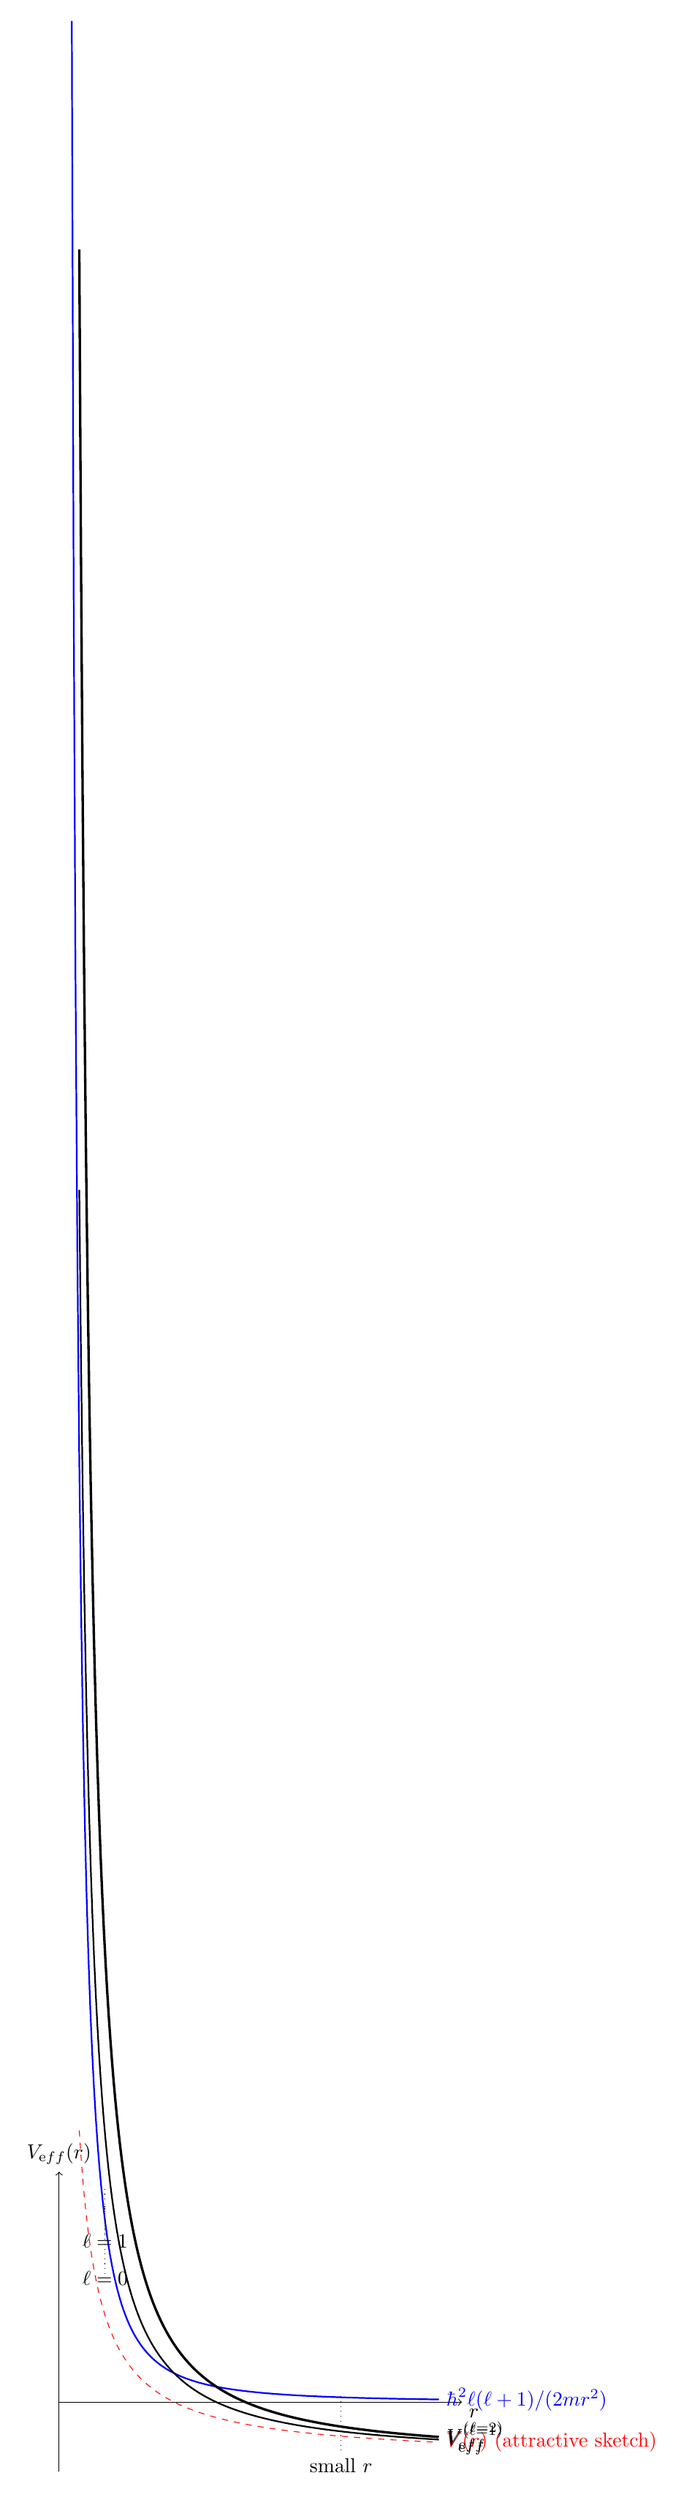
\begin{tikzpicture}[scale=1]
\draw[->] (0,0) -- (7.0,0) node[below right] {$r$};
\draw[->] (0,-1.2) -- (0,4.0) node[above] {$V_{\mathrm eff}(r)$};

\draw[blue, thick, domain=0.22:6.6,samples=200] plot ({\x},{2/(\x*\x)}) node[right] {\(\hbar^2\ell(\ell+1)/(2mr^2)\)};
\draw[red, thin, dashed, domain=0.35:6.6,samples=220] plot ({\x},{2/\x -1}) node[right] {\(V(r)\) (attractive sketch)};
\draw[thick, domain=0.35:6.6,samples=220] plot ({\x},{2/\x -1 + 2/(\x*\x)}) node[right] {\(V_{\mathrm eff}^{(\ell=1)}\)};
\draw[very thick, domain=0.35:6.6,samples=220] plot ({\x},{2/\x -1 + 4/(\x*\x)}) node[right] {\(V_{\mathrm eff}^{(\ell=2)}\)};

\draw[dotted] (4.9,0.1) -- (4.9,-0.9);
\node at (4.9,-1.1) {small \(r\)};

\draw[dotted] (0.8,3.0) -- (0.8,2.2);
\node at (0.8,2.15) {\(\ell=0\)};
\draw[dotted] (0.8,3.7) -- (0.8,2.9);
\node at (0.8,2.8) {\(\ell=1\)};
\draw[dotted] (0.8,3.4) -- (0.8,3.0);
\end{tikzpicture}
\caption{Frame 3: centrifugal repulsion and effective potential structure redrawn as TikZ, as presented by Susskind, lecture blackboard reconstruction. Caption type: re-rendered TikZ (from \texttt{lecture_03_frame_03.png}, due clarity normalization).}
\end{figure}

\paragraph{Interpretive note.}
Susskind emphasizes this is not a new postulate: it is the same classical decomposition viewed through conserved angular motion, then projected into a fixed-\(\ell\) quantum sector.

\begin{figure}[h]
\centering
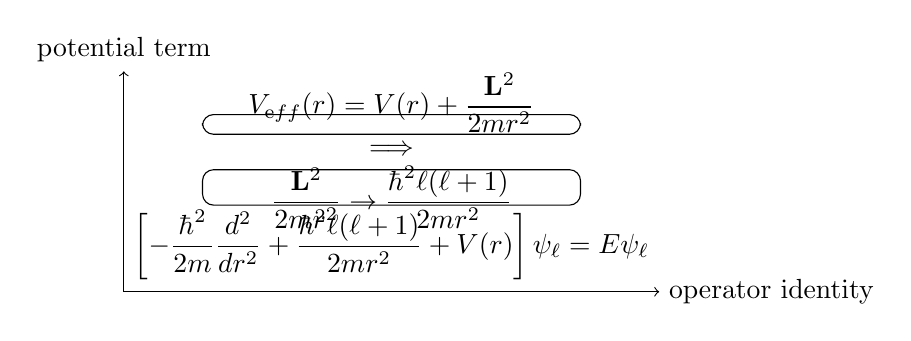
\begin{tikzpicture}[scale=1]
\draw[->] (0,0) -- (6.8,0) node[right] {operator identity};
\draw[->] (0,0) -- (0,2.8) node[above] {potential term};
\node at (3.4,2.4) {\(\displaystyle V_{\mathrm eff}(r)=V(r)+\frac{\mathbf L^2}{2mr^2}\)};
\node at (3.4,1.8) {\(\Longrightarrow\)};
\node at (3.4,1.2) {\(\displaystyle \frac{\mathbf L^2}{2mr^2}\to\frac{\hbar^2\ell(\ell+1)}{2mr^2}\)};
\draw[rounded corners] (1.0,2.0) rectangle (5.8,2.25);
\draw[rounded corners] (1.0,1.1) rectangle (5.8,1.55);
\node at (3.4,0.6) {\(\displaystyle \left[-\frac{\hbar^2}{2m}\frac{d^2}{dr^2}+\frac{\hbar^2\ell(\ell+1)}{2mr^2}+V(r)\right]\psi_\ell=E\psi_\ell\)};
\end{tikzpicture}
\caption{Frame 4: \(\mathbf L^2\to\hbar^2\ell(\ell+1)\) substitution and resulting effective radial term, as presented by Susskind, lecture blackboard reconstruction. Caption type: re-rendered TikZ (clarified from \texttt{lecture_03_frame_04.png}).}
\end{figure}

\section{Radial equation, nodes, and level organization by \(\ell\)}
For each \(\ell\), one solves the one-dimensional eigenproblem
\[
\left[-\frac{\hbar^2}{2m}\frac{d^2}{dr^2}+\frac{\hbar^2\ell(\ell+1)}{2mr^2}+V(r)\right]\psi_{n_r,\ell}(r)=E_{n_r,\ell}\,\psi_{n_r,\ell}(r).
\]
Node counting is the practical organizer:
\[
n_r=0,1,2,\dots,\qquad
E_{0,\ell}<E_{1,\ell}<E_{2,\ell}<\cdots
\]
for fixed \(\ell\), where \(n_r\) is the number of nodes of the radial solution in this sector. Each radial level at fixed \((n_r,\ell)\) carries \(2\ell+1\) magnetic states.

\begin{figure}[h]
\centering
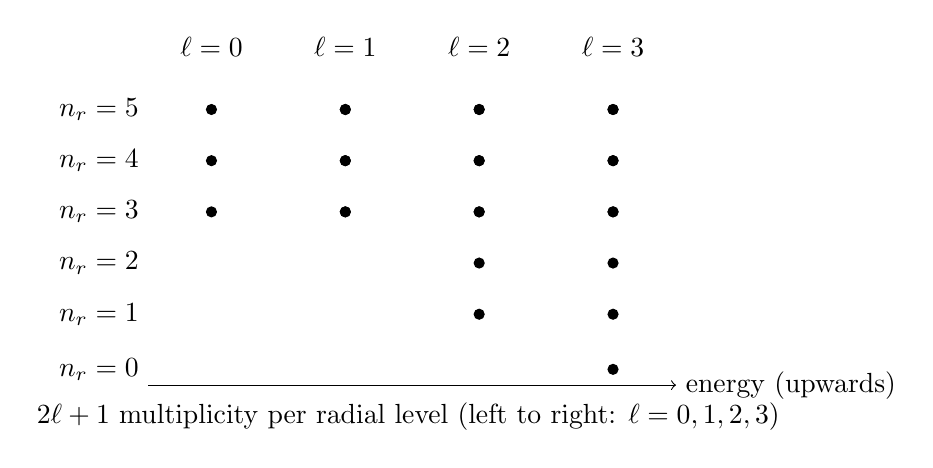
\begin{tikzpicture}[scale=1]
\foreach \x/\lab in {0.9/{\(\ell=0\)}, 2.6/{\(\ell=1\)}, 4.3/{\(\ell=2\)}, 6.0/{\(\ell=3\)}} {
  \node at (\x,2.9) {\lab};
}
\foreach \x in {0.9,2.6,4.3,6.0} {
  \foreach \y in {2.1,1.45,0.8} {
    \filldraw (\x,\y) circle (1.8pt);
  }
}
\foreach \x in {2.6} {
  \foreach \y in {2.1,1.45,0.8} {
    \filldraw (\x,\y+0.0) circle (1.8pt);
  }
}
\foreach \x in {4.3} {
  \foreach \y in {2.1,1.45,0.8,0.15,-0.5} {
    \filldraw (\x,\y) circle (1.8pt);
  }
}
\foreach \x in {6.0} {
  \foreach \y in {2.1,1.45,0.8,0.15,-0.5,-1.2} {
    \filldraw (\x,\y) circle (1.8pt);
  }
}
\draw[->] (0.1, -1.4) -- (6.8,-1.4) node[right] {energy (upwards)};
\foreach \y/\lab in {-1.2/{\(n_r=0\)}, -0.5/{\(n_r=1\)}, 0.15/{\(n_r=2\)}, 0.8/{\(n_r=3\)}, 1.45/{\(n_r=4\)}, 2.1/{\(n_r=5\)}} {
  \node[left] at (0.1,\y) {\lab};
}
\node at (3.4,-1.8) {\(2\ell+1\) multiplicity per radial level (left to right: \(\ell=0,1,2,3\))};
\end{tikzpicture}
\caption{Frame 5: schematic by-\(\ell\) ladder organization re-rendered in TikZ, indicating fixed-\(\ell\) node ordering and \(2\ell+1\) degeneracy at each radial level. Caption type: re-rendered TikZ (from \texttt{lecture_03_frame_05.png}).}
\end{figure}

\begin{figure}[h]
\centering

\includegraphics[width=\linewidth]{lecture_03_frame_05.png}
\caption{Frame 5 retained as visual reference for the by-\(\ell\) energy layout, as presented by Susskind, lecture blackboard reconstruction; redrawn version above reconstructs the same structure with consistent indexing.}
\end{figure}

\section{Hydrogen-like accidental structure and its limits}
For the nonrelativistic Coulomb potential, Susskind highlights the exceptional near-degeneracy:
\[
n=n_r+\ell+1,\qquad E_{n_r,\ell}\approx E_n\quad\Rightarrow\quad g_n=n^2 \ (\text{orbital multiplicity only}).
\]
This is specific to exact \(1/r\) symmetry and is not robust under realistic effects:
\[
\text{finite nucleus size, relativistic corrections, spin, and radiation/interaction effects break it.}
\]
Thus he treats this as an ``accidental'' (in the physical sense of fragile) degeneracy pattern, useful pedagogically but not final for real atoms.

Susskind then hands the narrative forward: in the next step the same algebraic motif is used for the harmonic oscillator.

\section{Setup-level harmonic oscillator handoff}
For a later section, the ladder construction reappears in
\[
H_{\mathrm{HO}}=\frac{p^2}{2m}+\frac12m\omega^2 x^2,\qquad
a=\frac{1}{\sqrt{2m\hbar\omega}}\bigl(m\omega x+ip\bigr),\quad
a^\dagger=\frac{1}{\sqrt{2m\hbar\omega}}\bigl(m\omega x-ip\bigr),
\]
\[
H_{\mathrm{HO}}=\hbar\omega\left(a^\dagger a+\frac12\right),\qquad
E_n=\hbar\omega\left(n+\frac12\right).
\]
This closes the lecture arc: angular-momentum ladder ideas and sectorization carry forward into oscillator quantization and beyond.

\section*{Summary}
The lecture’s architecture is now coherent as a single chain: angular-momentum algebra fixes multiplet structure and \((\ell,m)\) labelling; central symmetry implies \(2\ell+1\) degeneracy for fixed \(n_r,\ell\); fixed-\(\ell\) reduction turns the 3D problem into a radial one-dimensional equation with centrifugal term \(\hbar^2\ell(\ell+1)/(2mr^2)\). Node counting then orders energies within each \(\ell\)-sector, while hydrogen’s \(1/r\) potential adds an additional near-accidental \(n=n_r+\ell+1\) organization. The section closes by showing that ladder methods are the leitmotif, now passing naturally into harmonic oscillator operator methods.